\section*{Experiment 3: Verification of Thevenin’s theorem}  
\addcontentsline{toc}{section}{Experiment 3: Verification of Thevenin’s theorem}

\subsection*{Learning Objectives}
To verify Thevenin's theorem

\subsection*{Equipment:}

\begin{itemize}
    \item Voltmeter
    \item Ammeter
    \item Rheostats
    \item Connecting wires
    \item DC Power Supply
\end{itemize}

\subsection*{Statement:}
Thevenin’s theorem states that any linear two-terminal circuit can be replaced by an equivalent circuit consisting of a voltage source $V_{Th}$ in series with a resistor $R_{Th}$.

\vspace{0.25 cm}

\noindent \textbf{Thevenin's theorem} states that "Any linear circuit containing several voltages and resistances can be replaced by just one single voltage in series with a single resistance connected across the load." In other words, it is possible to simplify any electrical circuit, no matter how complex, to an equivalent two-terminal circuit with just a single constant voltage source in series with a resistance (or impedance) connected to a load. 

\vspace{0.25 cm}

\noindent \textbf{Thevenin’s equivalent circuit}

\begin{figure}[H]
    \centering
    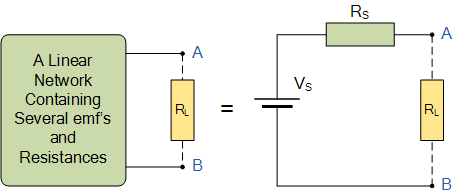
\includegraphics[width=0.7\linewidth]{img/thevenin.png}
    \caption{Thevenin's equivalent circuit}
    \label{fig:thevenin-circuit}
\end{figure}

\subsection*{Procedure:}

The voltage source is denoted by $V_{TH}$ (thevenin equivalentt voltage), and the resistor by $R_{TH}$(Thevenin resistor). The objective is to evaluate $V_{TH}$  and $R_{TH}$. The procedure of obtaining $V_{TH}$ and $R_{TH}$  is stated below for the circuits containing independent sources only. 

\begin{itemize}

    \item Remove the portion of the circuit external to which the Thevenin’s equivalent circuit is to be found. 
    
    \item Compute the voltage across the open-loop terminals. This voltage is $V_{OC}$. 

    \item Eliminate all the sources and compute the resistance across the open-loop terminal. This resistance is $R_{TH}$. A voltage source is eliminated by replacing it with a short circuit and a current source is eliminated by replacing it with an open circuit. 
    
    \item Draw the Thevenin equivalent circuit by placing the load resistor across the open-loop terminal 

\end{itemize}

\begin{figure}[H]
    \centering
    \includesvg[width=0.6\linewidth]{img/thevenin_eq.svg}
    \label{fig:thevenin_eq}
\end{figure}

\subsection*{Tabulation:}

\begin{table}[h]
    \centering
    \renewcommand{\arraystretch}{1.5} % Increases row height for better readability
    \begin{tabular}{c|p{3cm}|c|c|c|c|c|c}
        \hline
        \multirow{2}{*}{\textbf{S.No}} & \multirow{2}{*}{\makecell{\textbf{Supply} \\ \textbf{voltage (V)}}} & \multicolumn{3}{c|}{\textbf{MEASURED VALUES}} & \multicolumn{3}{c}{\textbf{THEORETICAL VALUES}} \\
        \cline{3-8}
        & & $V_{TH}$ (V) & $R_{TH}$ ($\Omega$) & $I_L$ (mA) & $V_{TH}$ (V) & $R_{TH}$ ($\Omega$) & $I_L$ (mA) \\
        \hline
        & & & & & & & \\
        \hline
    \end{tabular}
\end{table}

\subsection*{Calculation:}

Now the value of load current can be calculated as $I_{LC}$ = calculated value of $I_L  =  V_{TH} / (R_L + R_{TH})$

\vspace{0.25cm}

\noindent The value of $R_L$ can be calculated using the voltmeter and ammeter readings taken in step 2 of the procedure of $R_L = V/I$ of the procedure


\subsection*{Conclusion:}
By comparing the measured and theoretical values, verify the validity of Thevenin’s Theorem for DC circuits.

\newpage 